\section{Spatial \& Volumetric Normalization}
\label{sec:spatial}

\subsection{Raw Data Heterogeneity Analysis}
\label{sec:raw_heterogeneity}

Our cohort comprises 1,362 usable 3D volumetric scans (1 scan failed QC) from 15 acquisition centers. The raw data exhibits substantial heterogeneity:

\begin{figure}[H]
    \centering
    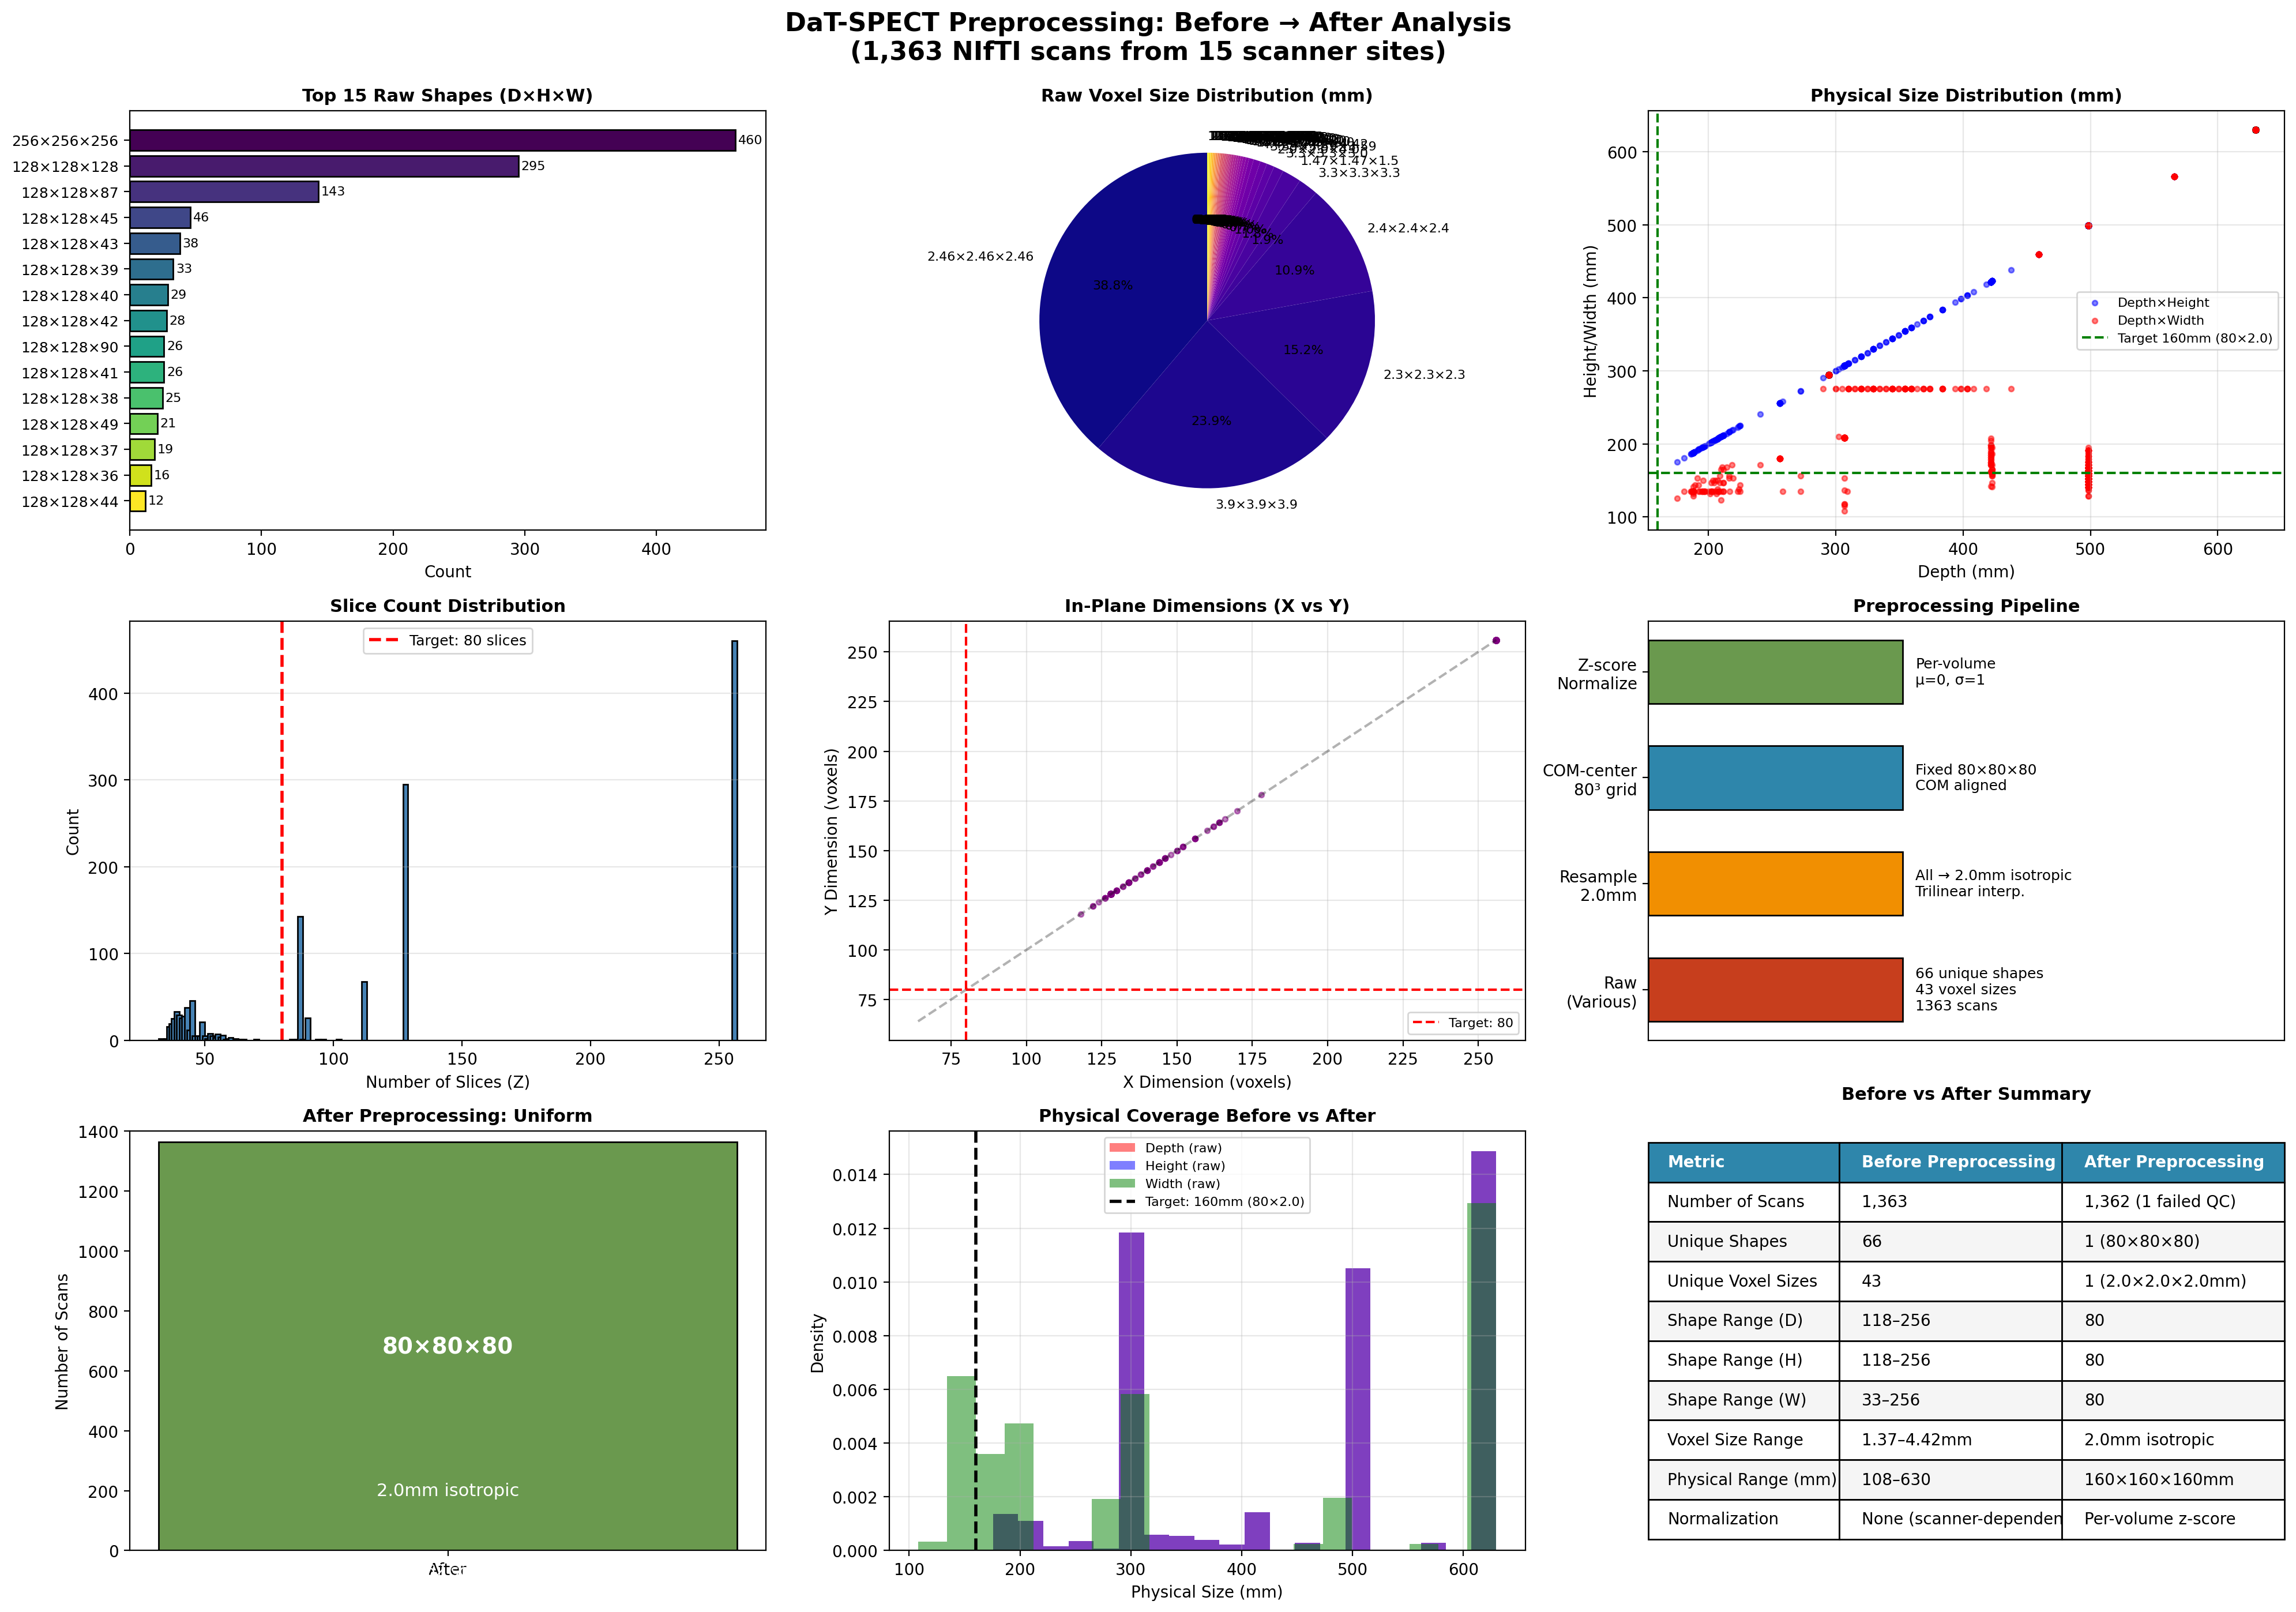
\includegraphics[width=0.95\linewidth]{figures/preprocessing_before_after.png}
    \caption{Before/after spatial standardization. (Top) Raw data diversity: 66 unique shapes, 66 voxel sizes, physical coverage 96--284~mm. (Middle) Pipeline stages. (Bottom) Uniform $80^3$ output at 2.0~\voxelunit~with summary statistics.}
    \label{fig:preprocessing}
\end{figure}

\begin{table}[H]
\centering
\caption{Raw dataset voxel size distribution (1,362 scans).}
\label{tab:voxel_dist}
\begin{tabular}{lccc}
\toprule
\textbf{Voxel Size (\ensuremath{\text{mm}^3})} & \textbf{Count} & \textbf{Percentage} & \textbf{Typical Matrix} \\
\midrule
2.46 $\times$ 2.46 $\times$ 2.46 & 528 & 38.8\% & 256$\times$256$\times$256, 128$\times$128$\times$128 \\
3.90 $\times$ 3.90 $\times$ 3.90 & 254 & 18.6\% & 128$\times$128$\times$128, 128$\times$128$\times$87 \\
2.30 $\times$ 2.30 $\times$ 2.30 & 130 & 9.5\%  & 134$\times$134$\times$112 \\
2.40 $\times$ 2.40 $\times$ 2.40 & 110 & 8.1\%  & 144$\times$144$\times$112 \\
Others (60 unique sizes) & 340 & 25.0\% & Various \\
\midrule
\textbf{Total} & \textbf{1,362} & \textbf{100\%} & \textbf{66 unique shapes} \\
\bottomrule
\end{tabular}
\end{table}

Physical field-of-view varies from 96~mm to 284~mm across dimensions (Figure~\ref{fig:preprocessing}, top-right). The two dominant resolutions (2.46~\voxelunit~and 3.90~\voxelunit) account for 57.4\% of scans.

\subsection{Preprocessing Pipeline}
\label{sec:preprocessing_details}

All scans undergo identical deterministic preprocessing:

\begin{enumerate}
    \item \textbf{RAS Reorientation:} NIfTI affine matrices reorient volumes to Right-Anterior-Superior coordinate space using nibabel's orientation transforms.
    \item \textbf{Isotropic Resampling:} Trilinear interpolation to 2.0~\voxelunit~isotropic. Per-dimension scale: $f_i = \text{voxel}_i / 2.0$.
    \item \textbf{Center-of-Mass Alignment:} COM of thresholded intensities ($>$5th percentile) translated to $80^3$ grid center (39.5). Affine: $\mathbf{T}(\mathbf{x}) = \mathbf{x} - \text{COM} + \mathbf{C}$.
    \item \textbf{Full Volume Retention:} Entire $80^3$ grid retained (no cropping) -- striatal signal spans full FOV in some acquisitions.
    \item \textbf{Per-Volume Z-Score Normalization:} $\tilde{v} = (v - \mu_v) / (\sigma_v + 10^{-8})$ computed independently per volume. Prevents dataset statistics from leaking into validation.
    \item \textbf{Inference Normalization:} Clip to [1st, 99th] percentile, min-max scale to [0, 1].
\end{enumerate}

\begin{table}[H]
\centering
\caption{Preprocessing summary: before vs. after.}
\label{tab:preprocessing_summary}
\begin{tabular}{lll}
\toprule
\textbf{Metric} & \textbf{Before} & \textbf{After} \\
\midrule
Scans & 1,363 & 1,362 (1 failed QC) \\
Unique shapes & 66 & 1 ($80\times80\times80$) \\
Unique voxel sizes & 66 & 1 (2.0~\voxelunit~isotropic) \\
Shape range (D/H/W) & 126--256 / 36--128 & 80 / 80 / 80 \\
Voxel size range & 1.47--3.90~\voxelunit & 2.0~\voxelunit \\
Physical coverage & 96--284~mm & 160$\times$160$\times$160~mm \\
Normalization & Scanner-dependent & Per-volume z-score \\
\bottomrule
\end{tabular}
\end{table}

\subsection{Grid Size Selection}
\label{sec:grid_size}

We evaluated input grid sizes at 2.0~\voxelunit~isotropic:

\begin{table}[H]
\centering
\caption{Input grid size ablation (Net3dR-v25, Fold 0).}
\label{tab:grid_ablation}
\begin{tabular}{cccc}
\toprule
\textbf{Grid} & \textbf{Voxel (\ensuremath{\text{mm}^3})} & \textbf{LogLoss} & \textbf{AUROC} \\
\midrule
64$^3$ & 2.5 & 0.289 & 0.951 \\
80$^3$ & 2.0 & \textbf{0.265} & \textbf{0.959} \\
96$^3$ & 1.67 & 0.271 & 0.956 (OOM) \\
\bottomrule
\end{tabular}
\end{table}

The $80^3$ grid at 2.0~\voxelunit~is the sweet spot: 64$^3$ loses anatomical detail; 96$^3$ exceeds 4GB VRAM even with gradient accumulation.